\hypertarget{sec:solution}{%
\chapter{Lowering the Initial Hurdle to Commence a Web Migration}\label{sec:solution}}
This chapter outlines the \gls{awsm} (Agile Web Migration for \glspl{sme}) \autocite{Heil2016AWSM} approach providing a solution to address the shortcomings identified in the state of the art of \gls{Web Migration} that keep \glspl{isv}, in particular \gls{sme}-sized \glspl{isv}, from commencing a \gls{Web Migration}.
To identify three main \textit{research objectives}, \cref{design-method-and-considerations} concretizes the effort and risk shortcomings identified in the state of the art by analyzing the stakeholder-specific situation in the thesis scenario.
\Cref{sec:solution-overview} derives the  \gls{awsm} solution achieving these research objectives, consisting of the \gls{awsm} Methodology and Toolsuite.

\hypertarget{design-method-and-considerations}{%
\section{Design Method}\label{design-method-and-considerations}}

This section describes the research methodology for designing the solution presented in \cref{sec:solution-overview}.
It 
\begin{itemize}
\item outlines the research process in \cref{sec:research-process},
\item presents problem analysis results in \cref{sec:problem-analysis-results}, and
\item derives the main research objectives in \cref{solution-research-design}.
\end{itemize}

We identified three main gaps in \gls{Web Migration} research with regard to \emph{effort and risk} in \cref{sec:sota.shortcomings}.
This section analyzes the resulting problems for \gls{sme}-sized \glspl{isv} with \glslink{Legacy System}{legacy}, non-\glslink{web}{web}, \gls{Desktop Application} products, and large existing user base introduced as main stakeholder in the thesis scenario in \cref{sec:scenario}.
It aims understanding the specific causes why \glspl{isv} are hesitant to commence a \gls{Web Migration} and what their the main concerns that create the organizational resistance are in order to devise a solution that addresses the research gaps in a suitable way for the main thesis stakeholder role.

The analysis follows the research process shown in \cref{fig:research-process} to systematically derive a suitable approach addressing concrete solution opportunities specified as research objectives.

Methods from two methodologies have been employed in this research process in addition to traditional requirements elicitation: \glslink{hcd}{Human-Centered Design} \footnote{cf.~\url{http://www.designkit.org/}} and \glslink{lfa}{Logical Framework Approach}\footnote{cf.~\url{https://ec.europa.eu/europeaid/multimedia/publications/publications/manuals-tools/t101\_en.htm}}.
These are briefly introduced and the application of methods is described in the following.

\textbf{\gls{hcd}} is a paradigm for designing solutions to problems with a focus on human needs and desires.
In this thesis, it is used as a tool for \emph{ideation}, that provides concrete guidelines and methods for conducting \emph{field research} in a design science context.
It has been defined with a technical scope for interactive systems and usability by \gls{iso} standard 9241-210 \autocite{ISO9241-210HCD}.
IDEO\footnote{\url{https://www.ideo.com/}}, one of the leading proponents and contributors of \gls{hcd} has assembled a systematic description of the methodology \autocite{HCD2015}.
The three-phase process comprises activities and artifacts that are used to get a deep understanding of problems from the human needs perspective, generate and select solution ideas and plan their implementation.

\glsunset{lfa}\textbf{\gls{lfa}} is a project planning and management methodology employed by the European Commission \autocite{Commission2004PCM} and other authorities.
In this thesis, it is employed as a tool for structuring observations gathered through \gls{hcd} methods into concrete problem descriptions in this thesis.
\gls{lfa} focuses on systematic \emph{problem and stakeholder analysis}, and \emph{objective setting} in the analysis stage.
In particular, \emph{\gls{lfa} problem trees} allow to identify and represent cause-effect-relationships in the problem domain and are used to analyze the situation of the thesis' main stakeholder, \glspl{isv} with \glslink{Legacy System}{legacy} software as characterized in \cref{sec:company-characteristics}.

\hypertarget{sec:research-process}{%
\subsection{Research Process}\label{sec:research-process}}
The research process comprises four phases:
\begin{itemize}
\item Field Research
\item Consolidation
\item Problem Analysis
\item Solution \& Research Design
\end{itemize}

Each phase is briefly described in the following.
An overview of the four-phase research process combining methods from \gls{hcd} and \gls{lfa} is presented in \Cref{fig:research-process}. \Cref{tbl:research-methods} provides a mapping of these methods on the phases.

\begin{figure}
\hypertarget{fig:research-process}{%
\centering
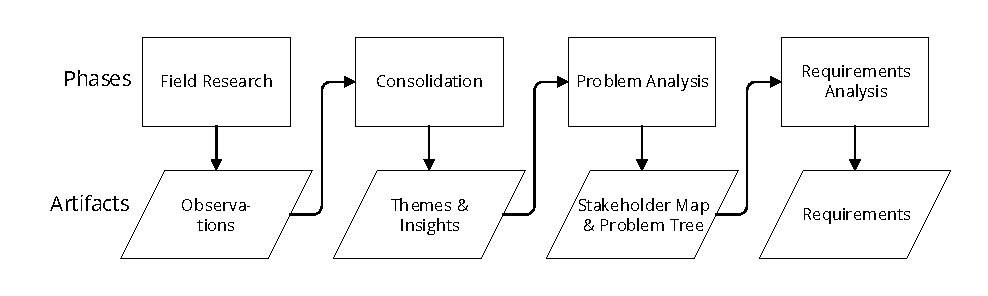
\includegraphics[width=0.99\textwidth]{../figures/20180115-DRF-Research-Process-Flow.pdf}
\caption{Solution and Research Design Process Flowchart}\label{fig:research-process}
}
\end{figure}

\hypertarget{tbl:research-methods}{}
\begin{longtable}[]{@{}ll@{}}
\caption{\label{tbl:research-methods}Methods used in Research phases}\tabularnewline
\toprule
\begin{minipage}[b]{0.28\columnwidth}\raggedright
Phase\strut
\end{minipage} & \begin{minipage}[b]{0.66\columnwidth}\raggedright
Methods\strut
\end{minipage}\tabularnewline
\midrule
\endfirsthead
\toprule
\begin{minipage}[b]{0.28\columnwidth}\raggedright
Phase\strut
\end{minipage} & \begin{minipage}[b]{0.66\columnwidth}\raggedright
Methods\strut
\end{minipage}\tabularnewline
\midrule
\endhead
\begin{minipage}[t]{0.28\columnwidth}\raggedright
Field Research\strut
\end{minipage} & \begin{minipage}[t]{0.66\columnwidth}\raggedright
\gls{hcd} Recruiting Tools, Interviews, Extremes and Mainstream, Immersion, Guided Tour\strut
\end{minipage}\tabularnewline
\begin{minipage}[t]{0.28\columnwidth}\raggedright
Consolidation\strut
\end{minipage} & \begin{minipage}[t]{0.66\columnwidth}\raggedright
\gls{hcd} Top Five, Find Themes, Create insight statements\strut
\end{minipage}\tabularnewline
\begin{minipage}[t]{0.28\columnwidth}\raggedright
Problem Analysis\strut
\end{minipage} & \begin{minipage}[t]{0.66\columnwidth}\raggedright
\gls{hcd} Create Frameworks, LFA Stakeholder Analysis, LFA Problem Tree\strut
\end{minipage}\tabularnewline
\begin{minipage}[t]{0.28\columnwidth}\raggedright
Solution \& Research Design\strut
\end{minipage} & \begin{minipage}[t]{0.66\columnwidth}\raggedright
\gls{hcd} How might we, Brainstorm, Get Visual, Prototyping, Feedback integration and iteration\strut
\end{minipage}\tabularnewline
\bottomrule
\end{longtable}

\textbf{Field research} was conducted at the headquarters of the \gls{sme}-sized \gls{isv} medatixx (cf.~\cref{sec:company-characteristics}) to elicit observations as basis for systematic problem analysis.
Several methods from \gls{hcd}'s Inspire phase were employed: \emph{Recruiting Tools} helped identify people to talk to, including senior management (``Leiter Softwareproduktion'' - Head of Development), middle management (``Abteilungsleiter Softwareproduktion'' - Head of Software Development Department) and staff (software engineers, software testers, scrum masters, product owners, DevOps, maintenance) and, following the \emph{Extremes and Mainstream} method including both proponents and opponents of \gls{Web Migration}.
A \emph{Guided Tour} was taken to get to know the different development teams, organizational structures, and work environment.
The observations were elicited using \emph{Interviews} in groups and single and using in-context \emph{Immersion}.
This method was particularly fruitful, comprising a one-week integration in a scrum team, actively participating in development activities and meetings.
This provided a good understanding of the daily development practice, expertise level of staff and a solid trust basis for interviews and subsequent feedback cycles.
More than 50 observations of the field research phase were captured and organized using Trello\footnote{\url{https://trello.com/}} cards.

\textbf{Consolidation} was used to abstract from the concrete observations into themes that capture relevant and recurring problem patterns.
This was supported by \gls{hcd}'s Ideation phase methods.
\emph{Find Themes} in combination with the collaborative filtering proposed in the \emph{Top Five} method was used to cluster the observations and identify the most relevant problem areas.
\emph{Insight statements} were created for the themes from observations.
The themes and insights were captured on post-its to provide the input for problem analysis.

\textbf{Problem Analysis} considered the relationships between the insights and themes to create a systematic view of the problem domain.
According to \gls{hcd}'s \emph{Create Frameworks} method, an initial relational map was created.
\gls{lfa} \emph{stakeholder analysis} was conducted to capture the stakeholder map which systematically describes characteristics and intentions of the involved roles.
The problem hierarchy was identified bottom-up from the insights and themes and their cause-effect relationships were represented as an \gls{lfa} \emph{problem tree}.
The results of the problem analysis phase were iteratively improved through a feedback loop with the \gls{isv} and are outlined in \cref{sec:problem-analysis-results}.

\textbf{Solution \& Research Design} transformed the problem analysis results into a solution design representing a set of research objectives.
A sub-tree of relevant problems according to the scope of this thesis \cref{sec:scope} was selected and \emph{How Might We} questions were formulated to drive ideation of opportunities (solution ideas) in the collaborative \emph{brainstorm} session.
To communicate the solution ideas, \emph{visual} representations (cf.~paper prototypes in \cref{sec:re.impl.integration}) and software \emph{prototypes} were created.
\emph{Feedback Integration and Iteration} was used to improve the opportunities through stakeholder feedback gathered in a presentation and discussion session at the \glspl{isv} headquarters and continued throughout the entire research project.
Eventually, partial research questions were derived which define the solution parts on a coarse-grain level.
The resulting solution \& research design is described in \cref{sec:solution-overview}.

\hypertarget{sec:problem-analysis-results}{%
\subsection{Problem Analysis Results}\label{sec:problem-analysis-results}}
Problem analysis conducted for this thesis comprises two parts: stakeholder analysis and problem tree analysis.
For stakeholder anlysis, we identified stakeholders and their characteristics in terms of their interests and how they are affected by a \gls{Web Migration}, their capacity and motivation, and possibilities to address and engage them.
For problem analysis, we identified stakeholder problems and their relationships.

\textbf{Stakeholder Analysis}.
\Cref{tbl:stakeholders} shows the results of stakeholder analysis.
The \gls{isv} stakeholder is further detailed in two distinct roles: \emph{Management} and \emph{Software Engineers}.
Management is responsible for the decision to migrate and is aware of the risks and thus must be addressed through \gls{risk management} and communication of benefits.
Software Engineers are the group of potential actors of \gls{Web Migration}; they define the requirements for migration activities through their expertise and development processes, and tailored methods need to be provided that reduce migration workload.
We use the term \emph{Migration Engineer} to refer to a Software Engineer who is performing \gls{Web Migration} activities.
Migration Engineers are to be considered a sub-class of Software Engineers, i.e.~all super-class characteristics apply.
Two customer stakeholders exist: the \emph{doctor's offices} are the direct customer of the \gls{pms} \gls{isv} whereas \emph{patients} are the customers of the customers and benefit the most from innovative features and improved usability and interactivity.
Furthermore, \emph{competitors} are affected by the effects on the market share of increased competitiveness of the \gls{isv} through \gls{Web Migration} and \emph{companies with similar situation}, i.e.~other \glspl{isv} with non-\glslink{web}{web}\glspl{Legacy System} and large user bases can benefit from the dissemination of results to apply to their situation.

\textbf{Problem Tree Analysis}.
The knowledge about the stakeholders together with themes and insights from the consolidation phase feeds into the analysis of problems and problem relationships.
The problem hierarchy is presented in \cref{fig:problem-tree}.
While it was created bottom-up, starting with insights, we briefly outline the problem tree top-down for easier understanding.
The arrows in the \gls{lfa} tree indicate cause-effect relationships, with effects represented in the direction of the arrows and causes in the opposite direction.
The root-level problem is the competitiveness of the \gls{isv}. Effects of this problem such as losing market shares to the competition are not shown for brevity.
This competitiveness is jeopardised by both the consequences of maintaining a \gls{Legacy System} and \gls{Technical Debt} (cf.~\cref{sec:situation}) leading to \emph{overloading} of staff and the \emph{hesitation to commence \gls{Web Migration}} due to \emph{doubts about feasibility and desirability} \autocite[cf.~also to resistance from organization in][]{Khadka2014ProfessionalsModernization,Sneed2010ReMiP}.
The \glslink{Legacy System}{legacy}-characteristic causes of overloading, such as low maintainability due to \emph{side-effects}, \emph{technological deprecation}, \emph{multi-platform environment} and \emph{limited time \& resources} are pushing factors in favour of a \gls{Web Migration}.
On the other hand, risk and effort of a \gls{Web Migration} constitute \emph{doubts about feasibility and desirability}.
In particular, \emph{limited time and resources} for conducting the migration, \emph{unknown plausibility of a \glslink{web}{web}-based version}, difficult \emph{integration into ongoing development}, and a \emph{lack of knowledge of methods and technologies} regarding migration and staff with \emph{\gls{Web Engineering} expertise} feed into feasibility doubts.
Likewise, \emph{lack of a deeper understanding of potential benefits}, the \emph{risk of losing poorly documented knowledge} and \emph{potential impact on existing customers} through abrupt changes form doubts about the desirability of \gls{Web Migration}.
The root causes on the lowest level of the problem tree are \emph{architectural degradation} of the \glspl{Legacy System}, \emph{missing documentation and experience of \glslink{Legacy System}{legacy} code}, a \emph{strict release cycle regime} due to regulatory and contractual constraints, lack of \emph{staff with \gls{Web Engineering} expertise} and a large existing \emph{customer base whose workflows are oriented on the user interaction of the software products}.
The latter three problems are situational problems that impose constraints on potential solutions as represented in requirements \cref{c:4} Agile, \cref{c:3} Exp and \cref{c:2} Reuse.

\begin{sidewaysfigure}
\hypertarget{fig:problem-tree}{%
\centering
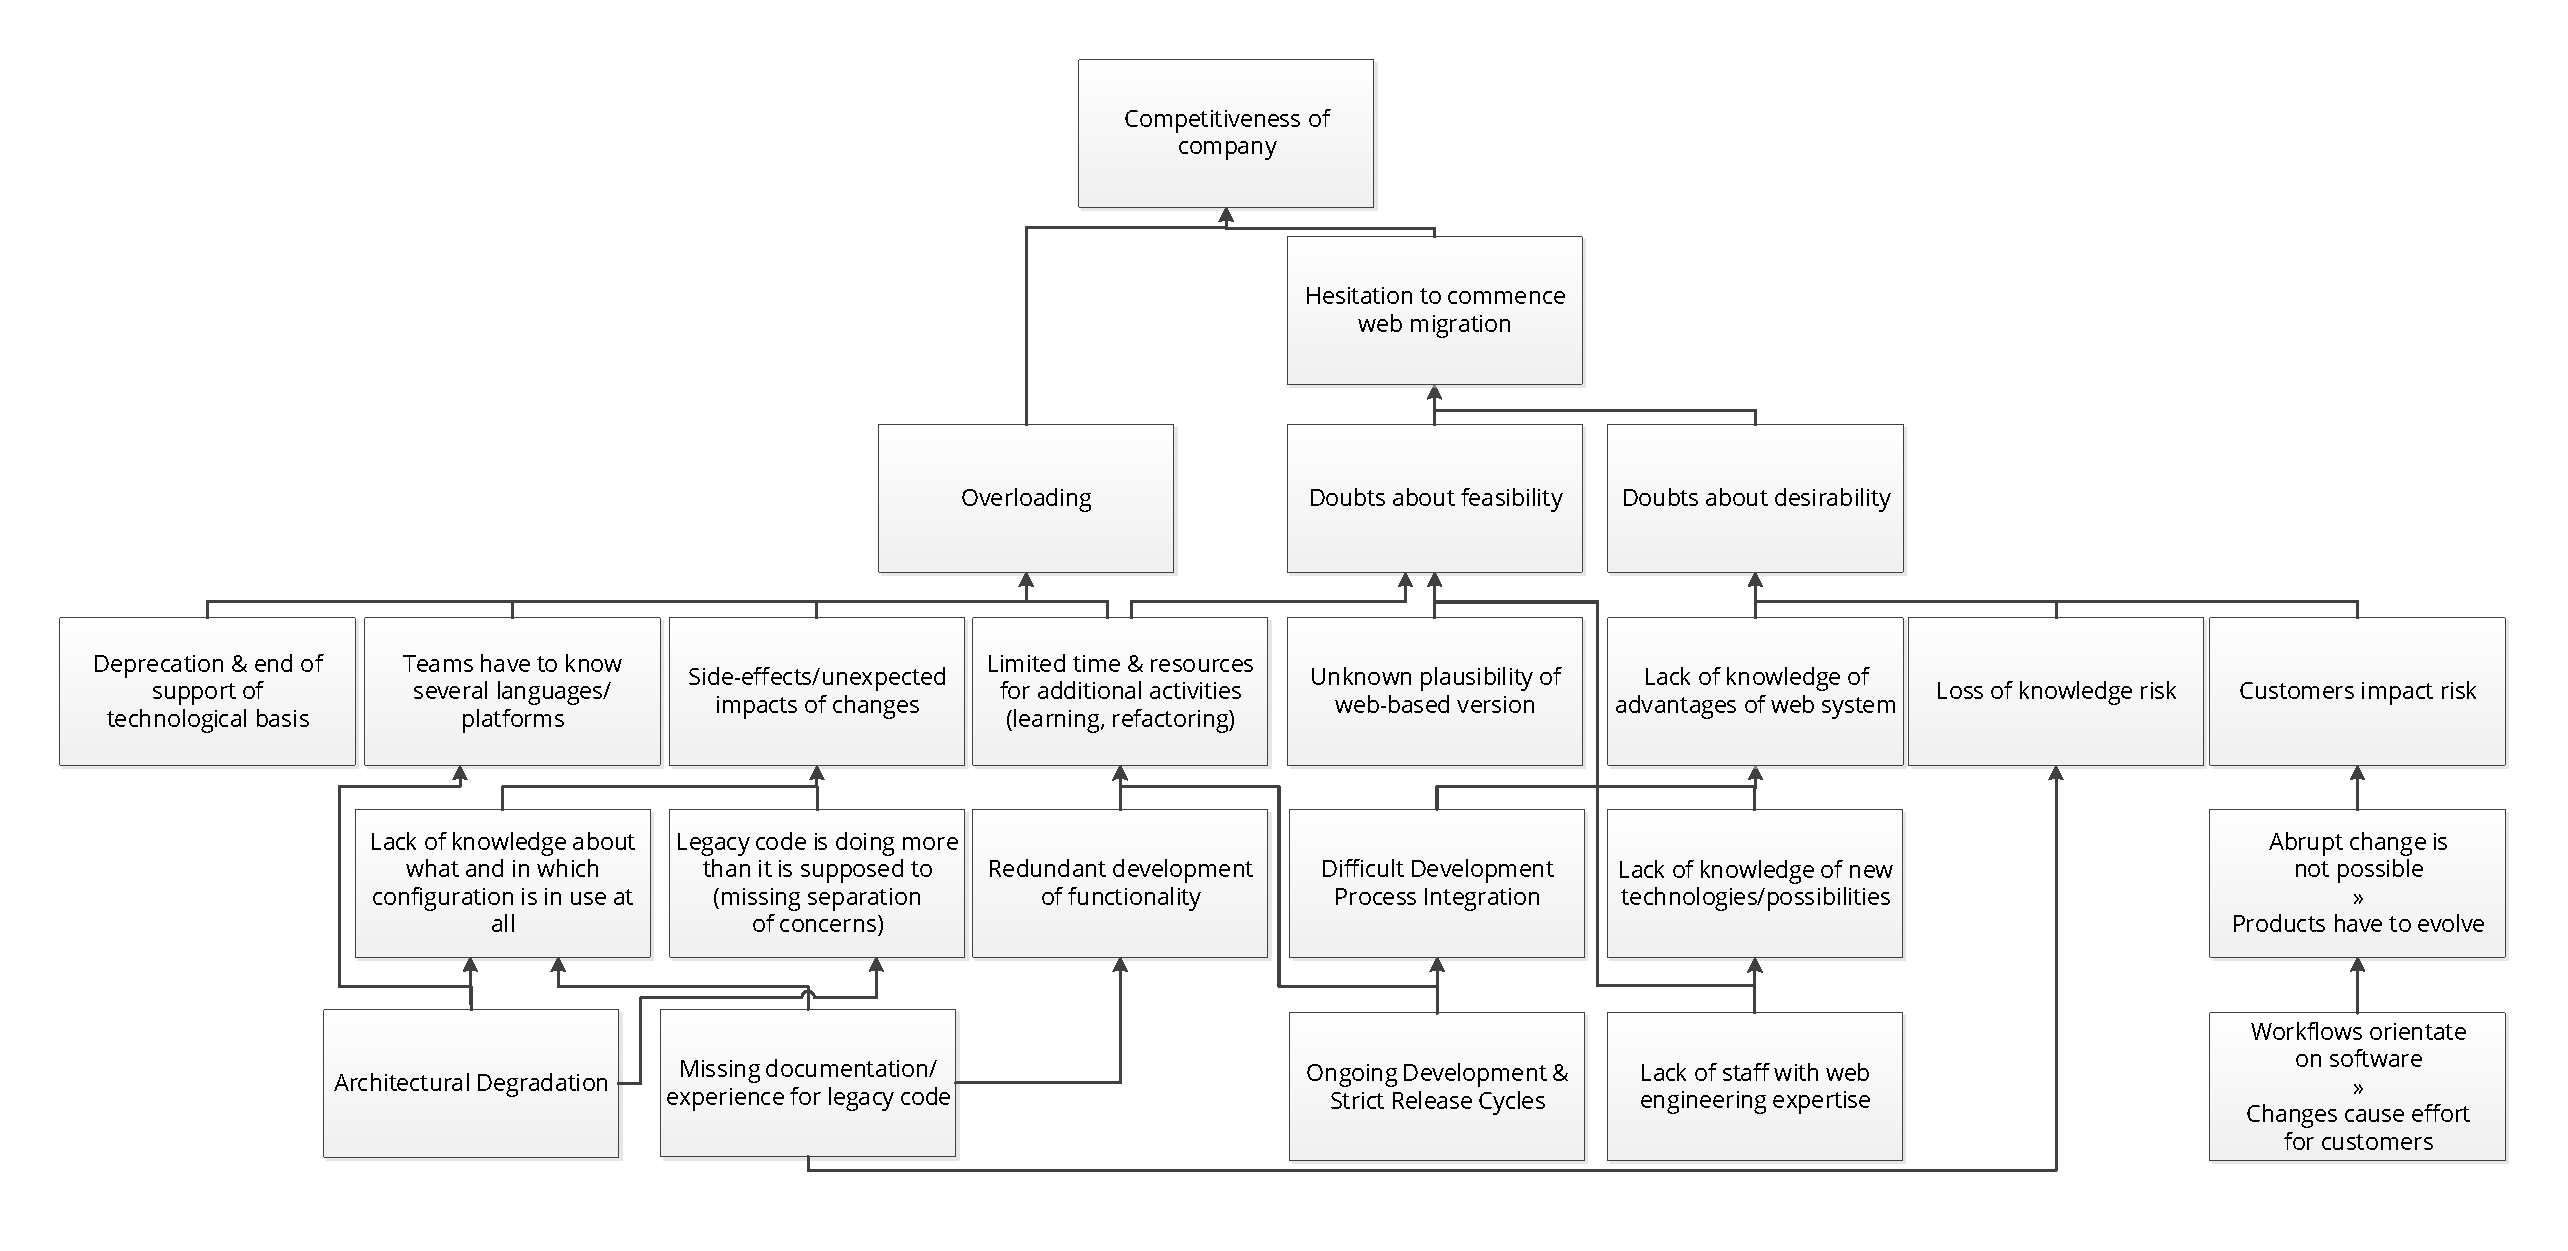
\includegraphics[width=0.99\textwidth]{../figures/20180115-DRF-Problem-Tree.pdf}
\caption{Hierarchical Representation of Problem Domain as LFA Problem Tree}\label{fig:problem-tree}
}
\end{sidewaysfigure}

\hypertarget{solution-research-design}{%
\subsection{Solution \& Research Design}\label{solution-research-design}}

This subsection derives the thesis' research objectives from the problems identified above.
The main research question of this thesis, \cref{rq:1}, directly corresponds to the \emph{hesitation to commence \gls{Web Migration}} problem and its corresponding sub-tree in \cref{fig:problem-tree}.
The detailed problem analysis shows that the \emph{effort and risk} factors described in the literature (cf.~\cref{sec:problem}) that make companies hesitant to commence a \gls{Web Migration} can be concretized into the problems of \emph{doubts about feasibility} and \emph{doubts about desirability} for \glspl{isv} with non-\glslink{web}{web}\glspl{Legacy System} and large existing user bases.
Through reformulation using the How-Might-We method of \gls{hcd}, the \gls{hmw} version of the initial research question RQ1

\begin{quote}
\emph{How might we support companies to commence \gls{Web Migration}?}
\end{quote}

translates into

\begin{quote}
How might we address IVS's doubts about feasibility and desirability?
\end{quote}

which defines the solution scope.
Aligned with the problem tree, this question is further broken down into the HMW questions listed in \cref{tbl:hmw}. 

\hypertarget{tbl:hmw}{}
\begin{longtable}[]{@{}ll@{}}
\caption{\label{tbl:hmw}How-Might-We-Questions for Ideation of Research Objectives}\tabularnewline
\toprule
\begin{minipage}[b]{0.06\columnwidth}\raggedright
ID\strut
\end{minipage} & \begin{minipage}[b]{0.88\columnwidth}\raggedright
Question\strut
\end{minipage}\tabularnewline
\midrule
\endfirsthead
\toprule
\begin{minipage}[b]{0.06\columnwidth}\raggedright
ID\strut
\end{minipage} & \begin{minipage}[b]{0.88\columnwidth}\raggedright
Question\strut
\end{minipage}\tabularnewline
\midrule
\endhead
\begin{minipage}[t]{0.06\columnwidth}\raggedright
HMW1\strut
\end{minipage} & \begin{minipage}[t]{0.88\columnwidth}\raggedright
How might reduce the risk of loss of knowledge through \gls{Web Migration}?\strut
\end{minipage}\tabularnewline
\begin{minipage}[t]{0.06\columnwidth}\raggedright
HMW2\strut
\end{minipage} & \begin{minipage}[t]{0.88\columnwidth}\raggedright
How might we demonstrate feasibility and advantages of a web-based version of the \gls{Legacy System}?\strut
\end{minipage}\tabularnewline
\begin{minipage}[t]{0.06\columnwidth}\raggedright
HMW3\strut
\end{minipage} & \begin{minipage}[t]{0.88\columnwidth}\raggedright
How might we reduce the risk of customers impact through \gls{Web Migration}?\strut
\end{minipage}\tabularnewline
\begin{minipage}[t]{0.06\columnwidth}\raggedright
HMW4\strut
\end{minipage} & \begin{minipage}[t]{0.88\columnwidth}\raggedright
How might we address HMW1, HMW2 and HMW3 with limited resources and lack of \gls{Web Engineering} expertise?\strut
\end{minipage}\tabularnewline
\bottomrule
\end{longtable}




Questions HMW1 - HMW3 address the problem sub-trees of feasibility and desirability doubts from a \emph{functional} \autocite{ISO/IEEE24765Vocabulary} perspective.
HMW4 is a \emph{non-functional} \autocite{ISO/IEEE24765Vocabulary} cross-cutting constraint, representing the resource and expertise problems in \cref{fig:problem-tree} and therefore is integrated with all following research objectives.

The overarching goal of this thesis is:

\begin{overarchinggoal}{og}
To provide methods, models, and tools that support \glspl{isv} with limited resources and lack of \gls{Web Engineering} expertise to commence a \gls{Web Migration}.
\end{overarchinggoal}

To achieve this objective, three specific research objectives were identified employing \gls{hcd}-based opportunity ideation described in \cref{sec:research-process}.
These objectives are:

\begin{researchobjective}{ro:1}
To provide a reverse engineering method, models and tools that allow to identify and manage existing knowledge in legacy source code with limited resources and lack of \gls{Web Engineering} expertise.
\end{researchobjective}

\begin{researchobjective}{ro:2}
To provide a \gls{risk management} method, models and tools that demonstrate desirability and feasibility of a potential \glslink{web}{web}-based version of the \gls{Legacy System} with limited resources and lack of \gls{Web Engineering} expertise.
\end{researchobjective}

\begin{researchobjective}{ro:3}
To provide an \gls{hci} method, models and tools to control the impact of \gls{Web Migration} on customers with limited resources and lack of \gls{Web Engineering} expertise.
\end{researchobjective}

These research objectives define the solution specified in the following section.

%\begin{figure}
%\hypertarget{fig:objectives}{%
%\centering
%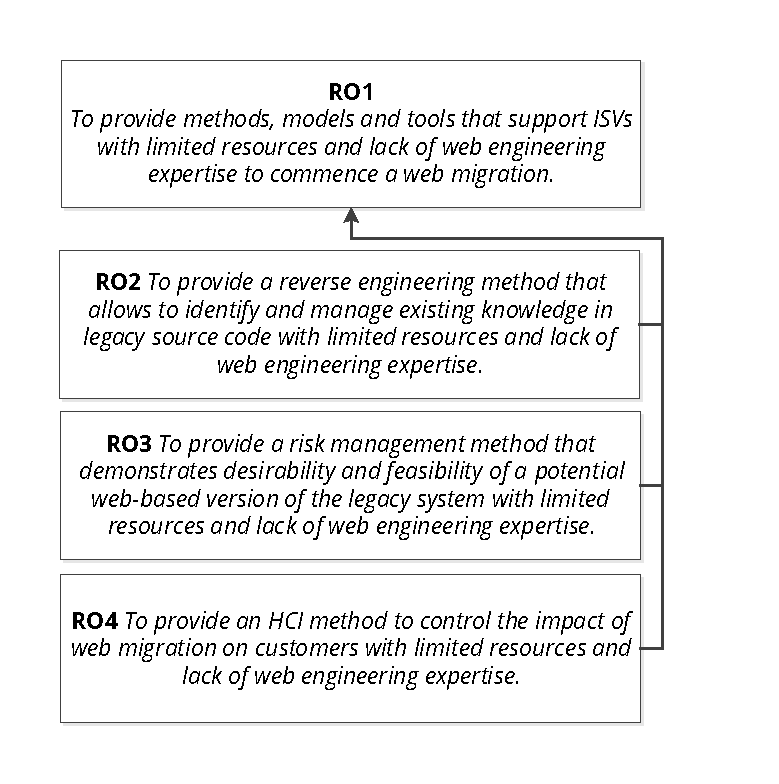
\includegraphics[width=0.99\textwidth]{../figures/objectives.pdf}
%\caption{Research Objectives}\label{fig:objectives}
%}
%\end{figure}

\hypertarget{sec:solution-overview}{%
\section{Agile Web Migration for SMEs}\label{sec:solution-overview}}

Our solution to address \cref{ro:1} to \cref{ro:3} is \emph{\gls{awsm} (Agile Web Migration for \glspl{sme})} \autocite{Heil2016AWSM}.
\gls{awsm} addresses shortcomings of existing \gls{Web Migration} approaches in initial phases of migration projects.

To achieve this, it provides solutions for each of the research objectives representing three methods:

\begin{itemize}
\item the \gls{awsm} reverse engineering method for \cref{ro:1},
\item the \gls{awsm} risk management method for \cref{ro:2}, and
\item the \gls{awsm} customer impact control method for \cref{ro:3}.
\end{itemize}


\gls{awsm} is structured according to the constructive elements of software engineering for quality ensurance \autocite{Wallmueller2001SoftwareQuality} into Principles, Formalisms, Methods, and Tools.
\Cref{fig:solution} shows the architecture of \gls{awsm}.

The Principles, Formalisms, Methods, and Tools are grouped into two main parts, the
\begin{itemize}
\item \emph{\gls{awsm} Methodology}, and the
\item \emph{\gls{awsm} Toolsuite}.
\end{itemize}


The \gls{awsm} Methodology describes \gls{awsm}'s Principles, Formalisms, and Methods.
The Tools supporting the \gls{awsm} Methodology constitute the \gls{awsm} Toolsuite.
Like other migration support methodologies  \autocite{Lewis2008SMART,Lewis2005SMART}, it does not impose a specific migration process.
Thus, the \gls{awsm} Methodology focuses on principles, formalisms, and methods for \gls{Web Migration} initiation and integration with existing comprehensive migration methods.
It can be combined with incremental reengineering and transformation processes.
\gls{awsm} addresses a package-oriented \autocite{Brodie1995Migrating} feature-driven \autocite{Menychtas2014ARTISTJournal} incremental process model.

We apply the \gls{remip} taxonomy  \autocite{Sneed2010SoftwareMigration} as shown in \cref{fig:methods-techniques-tools}, which divides \emph{migration processes} into distinct sequential or parallel \emph{migration phases}, throughout this thesis.
These phases comprise at least one \emph{migration activity} which employs one or more \emph{migration methods}.
The three \gls{awsm} methods described in the following are migration methods as they provide a conceptual model for conducting a migration activity.
For each \gls{awsm} method, at least one \emph{migration technique} is specified, detailing how to conduct a part of the method.
Each technique can be supported by a software implementation as \emph{migration tool}, which are the parts of the \gls{awsm} toolsuite.

\emph{Principles} are at the foundation of \gls{awsm}.
They are derived from the requirements and state of the art analysis results, and drive design decisions of the \gls{awsm} Methodology and Toolsuite.
\emph{Formalisms} form the conceptual basis for the methods and tools.
They specify the underlying mathematical model and semantics for knowledge in \glslink{Legacy System}{legacy} source code and the definition and algorithm for measuring the similarity between original and migrated user interfaces.
The following four subsections describe the solutions provided by the \gls{awsm} Methods, Principles, Formalisms, and Toolchain.

\begin{figure}
\hypertarget{fig:solution}{%
\centering
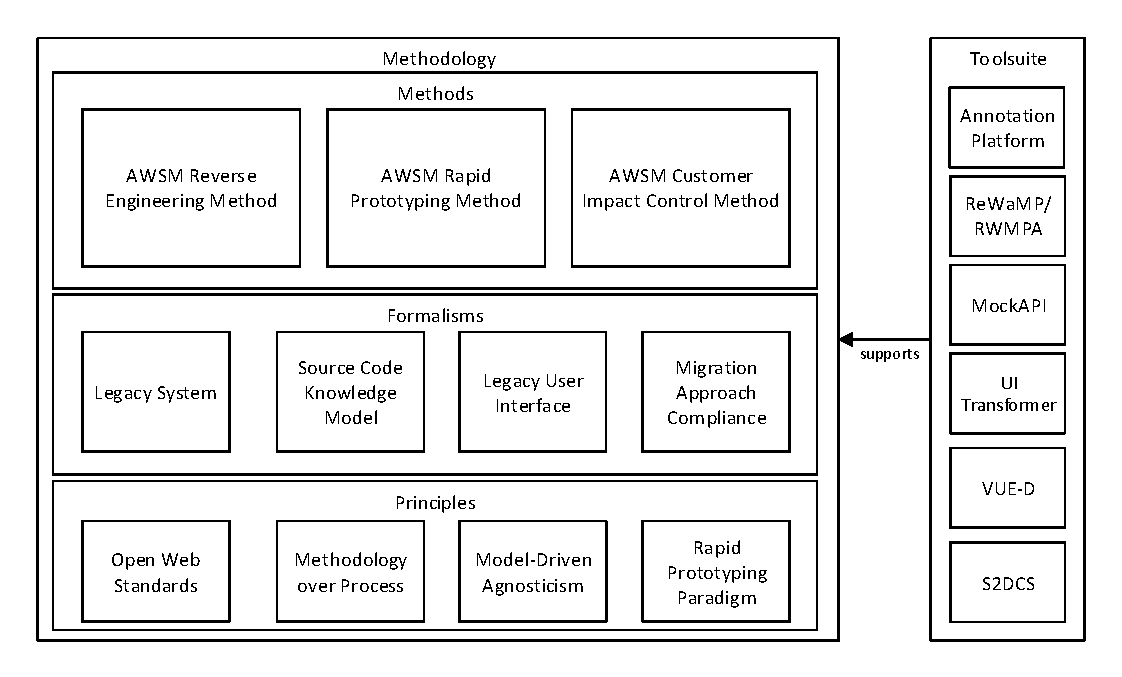
\includegraphics[width=0.99\textwidth]{../figures/solution.pdf}
\caption{AWSM Solution Overview}\label{fig:solution}
}
\end{figure}

\begin{figure}
\hypertarget{fig:methods-techniques-tools}{%
\centering
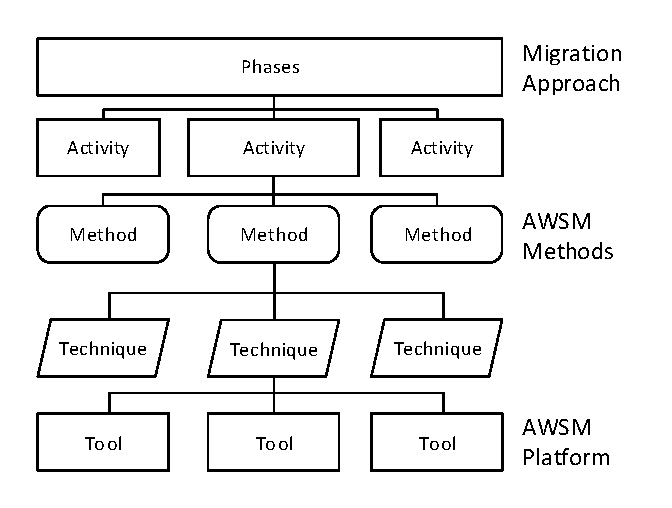
\includegraphics[width=0.7\textwidth]{../figures/remip-methods-techniques-tools.pdf}
\caption[AWSM mapped to \gls{remip} Taxonomy]{AWSM mapped to \gls{remip} Taxonomy \autocite[adapted from][]{Sneed2010SoftwareMigration}}\label{fig:methods-techniques-tools}
}
\end{figure}

\hypertarget{sec:solution.methods}{%
\subsection{AWSM Methods}\label{sec:solution.methods}}

To address research objectives \cref{ro:1}, \cref{ro:2}, and \cref{ro:3} respectively, \gls{awsm} provides the three methods:
\begin{itemize}
\item AWSM:RE -- the \gls{awsm} reverse engineering method,
\item AWSM:RM -- the \gls{awsm} risk management method,
\item AWSM:CI -- the \gls{awsm} customer impact control method.
\end{itemize}

These three methods provide techniques for solving the problems identified in \cref{sec:sota.shortcomings} in different  disciplines and phases of \gls{Web Migration}.
While the techniques of AWSM:RE and AWSM:RM belong to the earliest \gls{remip} phase, AWSM:CI techniques are conducted during Migration \& Transition.
The three methods cover several core and base disciplines each, but all are targeting the migration decision milestone.
\Cref{tbl:awsm-remip} provides a mapping of the \gls{awsm} methods onto the migration phases and disciplines of the Reference Migration Process \autocite{Sneed2010ReMiP} in order to facilitate integration with existing \gls{Web Migration} approaches. % as per principle \cref{p:2}.
The following three subsections outline the three AWSM Methods.

\hypertarget{awsm-reverse-engineering-method}{%
\subsubsection*{AWSM Reverse Engineering method}\label{awsm-reverse-engineering-method}}
\todo{figure}

The AWSM Reverse Engineering Method (AWSM:RE) provides a solution for \cref{ro:1} by specifying techniques to identify and manage problem and solution domain knowledge in \glslink{Legacy System}{legacy} source code.
AWSM:RE addresses the functional aspect of knowledge identification and management as well as the the non-functional constraint of limited resources and expertise of \cref{ro:1}.
The method extracts knowledge from \gls{Legacy System} \glspl{artifact} based on the conceptual models for a \gls{Legacy System} and knowledge in \glspl{Legacy System} introduced as formalisms in \cref{sec:formalisms}.
AWSM:RE solves \cref{ro:1} through
\begin{itemize}
\item a process for incremental knowledge extraction from legacy codebases
\item a queryable knowledge representation supporting \gls{Web Migration} processes based on reengineering or transformation at different degrees of model-driven adoption
\item a model for \glslink{Crowdsourcing}{crowdsourcing} reverse engineering activities
\end{itemize}

\par\smallskip
Knowledge extraction in AWSM:RE is solved through a \gls{Concept Assignment}-based reverse engineering technique.
It allows annotators to connect extracted knowledge to its distributed occurences in the legacy codebase.
AWSM:RE specifies a unified process model for human, automatic and crowd-based annotators.
The process model is incremental and integrated into ongoing development activities of \glspl{isv}.
The annotation process supports identification of relevant components for migration, elicitation of architectural knowledge and increasing decomposability of legacy code in the initial phase of \gls{Web Migration}.

AWSM:RE represents reverse-engineered knowledge in a queryable and interoperable way using semantic \gls{web} technologies to provide a basis for subsequent reengineering and transformation approaches.
Its \gls{owl}-Ontology for knowledge in legacy source code allows adaption of AWSM:RE to different \gls{Web Migration} methods at varying degrees of model-driven adoption.
The ability to query the reverse-engineered knowledge in a technology-independent graph-based form ensures applicability with a wide range of existing \gls{Web Migration} approaches and tools.

Unlike existing redocumentation and design recovery methods, AWSM:RE has a strong focus on applicability for \glspl{isv} with limited resources and limited \gls{Web Engineering} expertise.
To achieve this, AWSM:RE introduces the novel idea of \emph{crowdsourced reverse engineering} \autocite{Heil2018CSRE} and demonstrates applicability by re-formulating the problem of \gls{Concept Assignment} \autocite{Biggerstaff1994ConceptAssignmentJournal} as classification problem that can be solved using the \emph{\gls{Crowdsourcing} paradigm} \autocite{Howe2006}.
While \gls{Crowdsourcing} has seen adoption in forward software engineering, \gls{awsm} is the first approach to transfer the paradigm to reverse engineering for \gls{Web Migration}.
To make use of the benefits of the crowd with regards to workforce and expertise, AWSM:RE addresses the challenges of controlled disclosure and quality control.
%The concretization of the conceptual \gls{sckm} as \gls{owl}-Ontology allows adaption of AWSM:RE to different \gls{Web Migration} methods at varying degrees of model-driven adoption, according to principle \cref{p:3}.
AWSM:RE is described in detail in \cref{sec:awsm-re}.

\hypertarget{awsm-risk-management-method}{%
\subsubsection*{AWSM Risk Management method}\label{awsm-risk-management-method}}
\todo{figure}

The \gls{awsm} Risk Management method (AWSM:RM) provides a solution for \cref{ro:2} by specifying techniques to demonstrate desirability and feasibility of a potential \glslink{web}{web}-based version of the \gls{Legacy System}.
AWSM:RM addresses the functional aspect of desirability and feasibility demonstration as well as the the non-functional constraint of limited resources and expertise of \cref{ro:2}.
The method transforms existing software \glspl{artifact} defined in the conceptual model for a \gls{Legacy System} specified in \cref{sec:formalisms} into a running \glslink{web}{web}-based prototype.
AWSM:RM solves \cref{ro:2} through
\begin{itemize}
\item a process for rapid, semi-automatic creation of \glspl{web migration prototype}
\item a technique for business logic re-use in \glspl{web migration prototype} based on \glslink{wasm}{WebAssembly}
\item a technique for automatic transformation of legacy user interface to \glslink{web}{web}-based user interface prototypes
\end{itemize}

\par\smallskip
Unlike existing \gls{risk management} methods in the early stages of \gls{Web Migration}, AWSM:RM allows to create a concrete and tangible contribution to the \gls{business case} that serves as a means of communication for stakeholders to support decision making.
To achieve this, \gls{awsm} introduces the novel idea of \gls{Rapid Web Migration Prototyping} \autocite{Heil2018ReWaMP} by transferring the \emph{\gls{Rapid Prototyping} paradigm} \autocite{Gordon1995RapidPrototyping} from forward engineering into the \gls{Web Migration} domain.
AWSM:RM defines a process for rapidly creating \gls{Web Migration} prototypes based on the \gls{Legacy System} \glspl{artifact}.

To address the constraint of limited resources and \gls{Web Engineering} expertise in \cref{ro:2}, AWSM:RE leverages the thriving WebAssembly \gls{w3c} standard \autocite{W3C2018WebAssembly} to allow extensive re-use of existing business logic.
In this way, the semi-automated prototyping technique can be applied by  \gls{isv}'s existing staff with experience in the legacy technology.
Additional guidance is provided to reduce the required \gls{Web Migration} expertise.

For creating a \glslink{web}{web}-based user interface prototype, AWSM:RM allows to automatically transform legacy user interfaces based on an evolutionary optimization algorithm.
It addresses the challenge of mapping pixel-based legacy desktop user interface layouts to responsive grid layouts commonly used in \glspl{Web Application}.
AWSM:RM is described in detail in \cref{sec:awsm-rm}.

\hypertarget{awsm-customer-impact-control-method}{%
\subsubsection*{AWSM Customer Impact Control method}\label{awsm-customer-impact-control-method}}

The \gls{awsm} Customer Impact Control method (AWSM:CI) provides a solution for \cref{ro:3} by specifying techniques to control the impact of \gls{Web Migration} on the user bases of existing customers. % with limited resources and lack of \gls{Web Engineering} expertise.
AWSM:RM addresses the functional aspect of customer impact control as well as the the non-functional constraint of limited resources and expertise of \cref{ro:3}.
Based on the conceptual model of \glslink{Legacy System}{legacy} user interfaces specified in \cref{sec:formalisms}, AWSM:CI defines a visual similarity measure that allows determining and thus control the degree of visible changes introduced into the user interface through \gls{Web Migration}.
AWSM:CI solves \cref{ro:3} through
\begin{itemize}
\item a model for analysis of visual similarity between legacy \gls{Desktop Application} user interfaces and migrated \glslink{web}{web}-based user interfaces
\item a process for calibrating the similarity model with a limited number of users
\item a model for automatically detecting user interface elements
\end{itemize}

\par\smallskip
Unlike existing \gls{Web Migration} approaches, AWSM:CI explicitely addresses the concern of maintaining a similar look and feel beween legacy and migrated system by defining a visual \gls{ui} analysis model.
This model allows to compute a measure of visual similarity based on automatically detectable visual aspectsto resemble human perception of user interfaces.

To address the constraint of limited resources and \gls{Web Engineering} expertise in \cref{ro:3}, AWSM:CI avoids extensive empirical data collection with large numbers of test subjects and user interface combinations.
Instead, it specifies a process for calibrating the similarity model to the characteristics of the target user group with only a limited number of representatives and specifically designed test samples.
In this way, the similarity measurement can be calibrated with limited effort in initial migration phases and then automatically applied for large numbers of user interfaces created throughout \gls{Web Migration}.

The challenge lies in calculating object-dependent measures due to the heterogeneity of technologies and corresponding description formats for user interface elements.
While existing automatic analysis methods for \gls{web} user interfaces rely on DOM\footnote{Document Object Model, cf.~\autocite{W3C2015DOM}} analysis, the AWSM:CI similarity measure is applicable to both \glslink{Legacy System}{legacy} and \gls{web} user interfaces \autocite{Heil2016Similarity}.
To achieve this, AWSM:CI contributes to the novel field of research on visual analysis of user interfaces employing deep learning to automatically detect elements of the user interface enabling calculation of derivative object-dependent measures.
%Following principle \cref{p:1}, analysis results are made available using JSON.
AWSM:CI is described in \cref{sec:awsm-ci}.


\hypertarget{tbl:awsm-remip}{}
\begin{longtable}[]{@{}l@{\phantom{AAAAA}}l@{}l@{}l@{}}
\caption{\label{tbl:awsm-remip}Mapping of AWSM Methods to \gls{remip}}\tabularnewline
\toprule
\begin{minipage}[b]{0.07\columnwidth}\raggedright
\gls{awsm} Method\strut
\end{minipage} & \begin{minipage}[b]{0.18\columnwidth}\raggedright
Phase\strut
\end{minipage} & \begin{minipage}[b]{0.25\columnwidth}\raggedright
Core Disciplines\strut
\end{minipage} & \begin{minipage}[b]{0.39\columnwidth}\raggedright
Base Disciplines\strut
\end{minipage}\tabularnewline
\midrule
\endfirsthead
\toprule
\begin{minipage}[b]{0.07\columnwidth}\raggedright
\gls{awsm} Method\strut
\end{minipage} & \begin{minipage}[b]{0.18\columnwidth}\raggedright
Phase\strut
\end{minipage} & \begin{minipage}[b]{0.25\columnwidth}\raggedright
Core Disciplines\strut
\end{minipage} & \begin{minipage}[b]{0.39\columnwidth}\raggedright
Base Disciplines\strut
\end{minipage}\tabularnewline
\midrule
\endhead
\begin{minipage}[t]{0.07\columnwidth}\raggedright
AWSM:RE\strut
\end{minipage} & \begin{minipage}[t]{0.18\columnwidth}\raggedright
Preliminary Study\strut
\end{minipage} & \begin{minipage}[t]{0.25\columnwidth}\raggedright
Legacy Analysis, Requirements Analysis\strut
\end{minipage} & \begin{minipage}[t]{0.39\columnwidth}\raggedright
Configuration \& Change Management, Project Management, Migration Environment\strut
\end{minipage}\tabularnewline
\begin{minipage}[t]{0.07\columnwidth}\raggedright
AWSM:RM\strut
\end{minipage} & \begin{minipage}[t]{0.18\columnwidth}\raggedright
Preliminary Study\strut
\end{minipage} & \begin{minipage}[t]{0.25\columnwidth}\raggedright
Requirements Analysis, Target Design\strut
\end{minipage} & \begin{minipage}[t]{0.39\columnwidth}\raggedright
Project Management, Staff Qualification\strut
\end{minipage}\tabularnewline
\begin{minipage}[t]{0.07\columnwidth}\raggedright
AWSM:CI\strut
\end{minipage} & \begin{minipage}[t]{0.18\columnwidth}\raggedright
Migration \& Transition\strut
\end{minipage} & \begin{minipage}[t]{0.25\columnwidth}\raggedright
Target Design, Implementation\strut
\end{minipage} & \begin{minipage}[t]{0.39\columnwidth}\raggedright
Migration Environment\strut
\end{minipage}\tabularnewline
\bottomrule
\end{longtable}


\hypertarget{principles}{%
\subsection{AWSM Principles}\label{principles}}

The \gls{awsm} Methodology and Toolsuite is built on four principles.
These principles provide solutions to address the shortcomings in the state of the art of \gls{Web Migration} identified in \cref{sec:sota.shortcomings} that are cross-cutting non-functional concerns for each of the three research objectives.
Therefore, they drive design decisions of all methods and tools in the \gls{awsm} Methodology and Toolsuite.
The following \gls{awsm} Principles formulate four top-level design decisions of \gls{awsm} and their rationale:

\begin{thesisprinciple}{Open \gls{web} Standards}{p:1}
To address the problem of technology-specificity of \gls{Web Migration} approaches limiting their applicability and inhibiting interoperability, this principle advocates using and extending open \gls{web} standards in the \gls{awsm} Methodology and Toolsuite.
The use of standards is widely accepted in software engineering and \gls{Web Engineering}.
For \gls{Web Migration}, using in particular \gls{w3c} specifications and \gls{omg} migration standards allows interoperability with existing methods and tools and provides contributions that can easily be used and enhanced by future research (cf.~OpenStand Principles\footnote{\url{https://open-stand.org/about-us/principles/}}).
This especially applies to underlying data models, provided interfaces and technologies used in \gls{awsm}.
\end{thesisprinciple}

\begin{thesisprinciple}{Methodology over Process}{p:2}
To address the problem of a wide range of existing \gls{Web Migration} approaches with individual process models on the one hand, and their shortcomings with regard to \gls{Web Migration} initiation for \glspl{isv} with limited resources and lack of \gls{Web Engineering} expertise on the other hand, \gls{awsm} aims at providing a \emph{methodology} that addresses these shortcomings.
This principle advocates an integration with existing \gls{Web Migration} reengineering and transformation process models to prefer re-use over re-definition of a new \gls{Web Migration} process model.
Therefore, \gls{awsm} methods define mappings for extension of the most relevant \gls{Web Migration} approaches such as REMICS, ARTIST or UWA/UWAT+.
\end{thesisprinciple}

\begin{thesisprinciple}{Model-Driven Agnosticism}{p:3}
To address the limited applicability of web migration approaches due to the divide of the current \gls{Web Migration} landscape on the use of \gls{mde}, the \gls{awsm} Methodology and Toolsuite is agnostic to Model-Driven adoption.
This is required, since half of the approaches in \cref{sec:approaches}  employs \gls{mde} in some form, and half of the approaches does not.
Likewise, \gls{mde} practices are employed in varying degrees in forward \gls{Web Engineering} \autocite{Moreno2008MDWE}.
This principle advocates compatibility with Non-Model-Driven \gls{Web Migration} approaches as well as with \gls{Web Migration} approaches at different degrees of Model-Driven adoption.
In particular reverse engineering, which forms the basis of reengineering and transformation, is laid out agnostic but adaptable to concrete Model-Driven or Non-Model-Driven methods in \gls{awsm} to allow interoperability with a wide range of existing \gls{Web Migration} approaches.
\end{thesisprinciple}

\begin{thesisprinciple}{Rapid Prototyping Paradigm}{p:4}
To address the problem of a lack of demonstration of desirability for decision making in initial \gls{Web Migration} phases, this principle advocates applying the \gls{Rapid Prototyping} paradigm to the \gls{Web Migration} domain.
\gls{Prototyping} is an established means of improving quality in forward software engineering \autocite{Wallmueller2001SoftwareQuality}.
The \gls{Rapid Prototyping} paradigm \autocite{Gordon1995RapidPrototyping} with its dedicated focus on quick and cheap creation of tangible means of communication of envisioned software for all involved stakeholders \autocite{Alavi1984} has become particularly popular in the context of Agile Development \autocite{Abrahamsson2002Agile} and Human-Centered Design \autocite{HCD2015}.
Thus, the \gls{awsm} Methodology and Toolsuite favors the creation of prototypes as concrete, tangible means of communication to demonstrate desirability of a \glslink{web}{web}-based version of the migrated \gls{Legacy System} over theoretical and general argumentation and narrowly focused technical feasibility studies.
\end{thesisprinciple}

\hypertarget{sec:formalisms}{%
\subsection{AWSM Formalisms}\label{sec:formalisms}}

The \gls{awsm} Methodology provides solutions to \cref{ro:1}, \cref{ro:2}, and \cref{ro:3}.
These solutions are based on a common theoretical basis, the three \gls{awsm} Formalsisms specified in this subsection.
The formalisms define basic \emph{conceptual models} independent of their concrete implementation in the \gls{awsm} Toolsuite.
%The conceptual architecture of the \gls{awsm} toolsuite is discussed in \cref{sec:platform}.
\gls{awsm} defines three formalisms:
\begin{itemize}
\item Legacy System
\item Source Code Knowledge Model
\item Legacy User Interface
\end{itemize}
The \gls{Legacy System} formalisms defines a \gls{Legacy System} in terms of its \emph{software \glspl{artifact}} \autocite{OMG2016KDM}, i.e.~of physical resources that are available as inputs for analysis and transformation activities described in the methods of the \gls{awsm} methodology.
The Source Code Knowledge Model formalism defines the knowledge contained in a \gls{Legacy System} in terms of relevant \emph{software assets} \autocite{OMG2016KDM} that are represented through the \glspl{artifact} but not necessarily existing in explicit forms.
The Legacy User Interface formalism defines a uniform description of user interfaces and their conceptual components to support \gls{awsm}'s focus on maintaining user interface consistency across legacy and target technologies.

As a design decision reasoned in principle \cref{p:1}, AWSM Formalisms extend \gls{omg}'s Knowledge Discovery Meta-Model specification.
On the one hand, this allows \gls{awsm} to re-use the semantics specified in \gls{kdm} and avoid lengthy descriptions and re-definitions.
On the other hand, \gls{kdm}'s technical focus on file-based knowledge representation is insufficient for the \gls{awsm} Methodology.
Therefore, \gls{awsm} makes use of \gls{kdm}'s extension mechanism to effectively use only parts necessary \autocite{OMG2016KDM} for the \gls{awsm} Methods and adds the required missing semantics.
For brevity, when referring to \gls{kdm} in the following description of formalisms, these references are to be considered as a reference to \gls{kdm} version 1.4 of September 2016 \autocite{OMG2016KDM}.


\subsubsection*{\gls{Legacy System}}
The \gls{Legacy System} formalism specifies the conceptual model of the central object of investigation of this thesis and is used to describe the source material of all \gls{awsm} Methods and Tools.
%A \gls{Legacy System} is the basis for any \gls{Web Migration} and the central object of investigation of this thesis, serving as the starting point for the three \gls{awsm} methods.
\gls{kdm} \autocite{OMG2016KDM} provides a comprehensive \emph{\gls{metamodel}} for describing \glspl{Legacy System}.
\gls{awsm}'s conceptual model of a \gls{Legacy System} is based on a subset of \gls{kdm} concepts which provides the common foundation for the understanding of \glspl{Legacy System} in the context of the \gls{awsm} Methodology.
In particular, the \emph{inventory model} of the \gls{kdm} \emph{source package}, the \emph{platform package} and the \emph{\gls{ui} package} are relevant for \gls{awsm}.
In \gls{awsm}, a \gls{Legacy System} \(\mathfrak{L}\) is a 6-tuple:

\begin{equation}\mathfrak{L} = (B, Dep, \underline D,  E, D, U)\label{eq:legacy-system}\end{equation}

\(B\) is the \glslink{Legacy System}{legacy} codebase consisting of a set of source code files (\gls{kdm}: SourceFile), configuration files (\gls{kdm}: \emph{ConfigFile}) and other textual documents (\gls{kdm}: \emph{Document}).
\(Dep\) are the dependencies of the \gls{Legacy System} (\gls{kdm}: \emph{LinkableFile}), in particular third-party libraries (\gls{kdm}: \emph{LibraryFile}).
The dependency matrix \(\underline D: \{1,\ldots, |B|\} \times \{1,\ldots, |Dep|\} \mapsto [0,1]\) is a binary matrix with \(\underline D_{i,j} = 1 \Longleftrightarrow f_i \in B\) depends on \(dep_j \in Dep\), else \(\underline D_{i,j} = 0\).
\(E\) are the executables (\gls{kdm}: \emph{ExecutableFile}) of the \gls{Legacy System}.
In some scenarios \(B\) or \(E\) can be \(B=E=\emptyset\) \autocite{Binkley2007b}, however, as described in \cref{sec:scenario-code}, we assume availability of source code and executables in this thesis.
\(D\) represents the persistent data of the \gls{Legacy System} such as databases, storage files (\gls{kdm}: \emph{FileResource}), XML or JSON files.
\(U\) is the set of resources that form the user interface (\gls{kdm}: \emph{UIModel}) of the \gls{Legacy System}, consisting of container resources (\gls{kdm}: \emph{UIResource}) like screens.
The elements of \(U\) are not identical to their formal representation in \(B\) (e.g.~XAML files, \gls{mfc} resource files), but they are resulting from it and part of the executables in \(E\) from where their visual (i.e.~pixel-based) representation can be retrieved.
The \glslink{Legacy System}{legacy} user interface is described in more detail in \cref{sec:ui-formalism}.


\subsubsection*{Source Code Knowledge Model}
To achieve \cref{ro:1}, the risk of losing knowledge through \gls{Web Migration} needs to be addressed by extracting, capturing and preserving valuable knowledge in the \gls{Legacy System}.
The \gls{sckm} formalism is the part the \gls{awsm} solution that allows to represent arbitrary knowledge in \glspl{Legacy System}.
%The \gls{sckm} is at the core of the \gls{awsm} reverse engineering method.
%As argued in the introduction, \glspl{Legacy System} contain valuable \emph{knowledge from the problem and solution domain} \autocite{Marcus2004ProblemLocation} that must be preserved throughout migration.

The challenge addressed by the \gls{sckm} is the implicit nature of knowledge in \glslink{Legacy System}{legacy} code bases: similar to \emph{tacit knowledge} in organizations which is
not expressed explicitly but guides human behavior \autocite{Nonaka2008TacitKnowledge}, the knowledge in \glspl{Legacy System} is not explicitly documented but governs how they operate.
Codification \autocite{Hansen1999KnowledgeManagement} is required to make it explicit, which is achieved through \emph{reverse engineering}.
The knowledge reverse-engineered from the \glslink{Legacy System}{legacy} source code through redocumentation and design recovery needs to be represented at different levels of abstraction \autocite{Chikofsky1990ReverseEngineering} and stored in a \emph{knowledge base} \autocite{ISO/IEEE24765Vocabulary} to feed into subsequent reengineering or transformation.


\gls{omg}'s \gls{kdm} is insufficient for describing implicit knowledge.
%provides a basic model for \glslink{Legacy System}{legacy} source code knowledge above procedure level in the \gls{kdm} specification as described in \cref{sec:adm}.
%Thus it is used as the basis for the \gls{sckm}.
It is focused on redocumentation knowledge, i.e.~equivalent representations of knowledge within the same abstraction level, the implementation level \autocite{Chikofsky1990ReverseEngineering}, describing the structure of the \glslink{Legacy System}{legacy} codebase in terms of modules, classes, methods, files.
\gls{kdm} assumes knowledge to reside in dedicated files -- data in data files, configuration in configuration files, etc.
-- whereas knowledge often appears mixed, due to the missing separation of concerns in \glspl{Legacy System}, within the source code.

Therefore, the \gls{sckm} allows the representation of design recovery knowledge, i.e.~knowledge on higher levels of abstraction, free of the assumption of explicit representation while maintaining the connection to its occurrence in structural parts of the source code.
The \gls{sckm} formalism specifies two conceptual models:
\begin{itemize}
\item a unified knowledge model independent of explicit physical representations
\item a model for linking knowledge to its occurences within artifacts of the legacy code
\end{itemize}

\textbf{Unified knowledge model.} In \gls{awsm}, an instance of knowledge \(k\) in the \gls{Legacy System} \(\mathfrak{L}\) is a tuple

\begin{equation}k = (t, r)\label{eq:knowledge}\end{equation}

of type \(t \in T\) and a representation \(r\).
%
%Types
%Migration aims at retaining the functionality of \glspl{Legacy System} in new environments \autocite{Bisbal1999LegacyInformationSystems}, with functionality referring to domain knowledge and business logic \autocite{Wagner2014}.
There are two basic varieties of knowledge in \glslink{Legacy System}{legacy} source code:
\begin{itemize}
\item \emph{Features} describe functionality of the \gls{Legacy System} (What) and can be represented as user stories, scenarios, use cases etc.
\item \emph{Domain knowledge} is the knowledge supporting the implementation of features, describing parts of the problem and solution domain of the \gls{Legacy System} (How).
\end{itemize}
Domain knowledge is divided into problem and solution domain knowledge \autocite{Marcus2004ProblemLocation}.
Problem domain knowledge comprises business processes and business rules.
Solution domain knowledge comprises presentation, persistence, algorithms, configuration, deployment and explanatory\footnote{natural-language knowledge embedded in the code as comments}.
\gls{sckm} exceeds the classical three-tier-architecture perspective considered in program decomposition providing a more detailed distinction of domain knowledge in the legacy source code.
%Typically, three categories corresponding to a classical three-tier-architecture are considered in program decomposition: \emph{presentation} (\gls{kdm} \emph{\gls{ui} domain}), \emph{application logic} (\gls{kdm} \emph{ConceptualFlow}) and \emph{persistence} (\gls{kdm} \emph{data domain}) \autocite{Canfora2000Decomposing}.
%Presentation comprises information about the user interface layout and the user interaction handling.
%Persistence defines knowledge about data models, data flow, caching, etc.
%The \gls{sckm} extends the three basic categories allowing a more detailed distinction of domain knowledge in the source code.

%In particular, \emph{business processes} and \emph{business rules} (\gls{kdm} \emph{RuleUnit}) \autocite{Aversano2001,Sneed2010SoftwareMigration,Wagner2014,Ulrich2011} are crucial problem domain knowledge.
%Solution domain knowledge comprises \emph{algorithms} (\gls{kdm}: \emph{BehaviorUnit}), \emph{configuration} (\gls{kdm}: \emph{ConfigFile}) and \emph{deployment} (\gls{kdm}: \emph{Deployment}).
%Note that both business processes and algorithms describe processes in the source code, but business processes are processes that exist in the problem domain whereas algorithms are solution domain processes.
%Furthermore, \glspl{Legacy System} can contain \emph{explanatory} natural-language knowledge embedded in the code as comments (\gls{kdm}: \emph{CommentUnit}).
%A similar distinction can be found in the taxonomy of \glslink{Legacy System}{legacy} artifacts in ARTIST \autocite{ARTIST2013Taxonomy}.

%Representations
These knowledge types can be represented by a variety of representations like \gls{uml} class diagrams, \gls{bpmn} diagrams, flow charts, SBVR\footnote{\url{https://www.omg.org/spec/SBVR/}} rules, other forms of models, informal or semi-formal natural language texts etc., depending on the intended use and can even have no representation (\(r=0\)) since determination of the type of a particular piece of \(\mathfrak{L}\) is knowledge.

\textbf{Linking knowledge to legacy code.} As knowledge is implicitly represented and distributed (e.g.~partial classes) in the source code, it is crucial to codify the connection to its occurrences in the source, in particular considering the importance of decomposability and traceability for migration.
\gls{awsm} models this connection as \emph{annotation} \(a \in K^* \times L^*\):

\begin{equation}a = (k, l)\label{eq:annotation}\end{equation}

The annotation \(a\) represents the \emph{intension} and \emph{extension} \autocite{Chen2010FeatureLocation} of knowledge: it associates a piece of knowledge \(k\) with its location \(l\) in the \glslink{Legacy System}{legacy} code base.
While \gls{kdm} relates knowledge to physical \glspl{artifact} like files and structural elements like classes, the \gls{sckm} considers knowledge to be an independent \gls{asset} that can be related to arbitrary parts within the elements of \(\mathfrak{L}\).
%The \emph{location} \(l\) can be specified as a reference to a specific segment of code \(s\) within a physical source code \gls{artifact} \(f \in B\) of the \glslink{Legacy System}{legacy} codebase.
%The source file content is interpreted as linear stream of characters, allowing to define a segment in terms of inclusive start \(\alpha\) and end \(\omega\) position in that stream:

Based on this model, we define the reverse engineering method of \cref{ro:1} as the application of a function \(re: B^* \mapsto A^*\) that maps a \glslink{Legacy System}{legacy} codebase \(B\) onto a set of annotations \(A = \{a_1,a_2,\ldots,a_n\}\): \(re(B) = A\), identifying a set of knowledge instances \(K\in K^*\) and their occurrences \(L \in L^*\) in the source code.
The information forms the \emph{legacy code knowledge base} \(\mathbb{K}_{B}\):

\begin{equation}\mathbb{K}_{B} = (K, A)\label{eq:knowledgebase}\end{equation}

%\Cref{sec:awsm-re} describes the interoperable and queryable implementation of \(\mathbb{K}\) through ontological modeling of the \gls{sckm} using semantic \gls{web} technologies.

\hypertarget{sec:ui-formalism}{%
\subsubsection*{Legacy User Interface}\label{sec:ui-formalism}}
To achieve \cref{ro:2} and \cref{ro:3}, \gls{awsm} addresses the lack of user interface migration and user interaction re-use of existing \gls{Web Migration} approaches as identified in \cref{g:3}.
This requires a formalism as common conceptual model for describing the \glslink{Legacy System}{legacy} user interface and its migrated derivatives.
%The user interface is an essential concern of \gls{Web Migration} since migration from a \glslink{Desktop Application}{desktop} \gls{gui} to a \glslink{web}{web}-based \gls{gui} rendered in the browser visibly changes the ``\emph{look and feel}'' \autocite{Rodriguez-Echeverria2012MIGRARIA,Lucia2008,Distante2002} and impacts existing users.
%This formalism defines a conceptual model of the \glslink{Legacy System}{legacy} user interface that serves as the basis for the \gls{awsm} customer impact control method.
User interfaces are defined in terms of Task, Behavior, Thesaurus, Layout and Material \autocite{Bakaev2017Kansei}.
The \gls{awsm} conceptual model of legacy user interfaces focuses on the layout aspect, because of three reasons: 1. the layout necessarily undergoes the most visible change through \gls{Web Migration}, whereas changes in e.g.~Task or Thesaurus can be avoided, 2. it is the basic design \gls{artifact} of the new \gls{web} \gls{ui}, influencing other aspects like Behavior and 3. it has the most degrees of freedom during re-design, in contrast to e.g.~Material which is governed by the platform.

\gls{awsm} defines a concrete \glslink{Legacy System}{legacy} user interface \(u \in U\) from the 
set of resources that form the user interface of the \gls{Legacy System} as
%i.e.~top-level \gls{ui} container elements without parents like screens, windows, dialogues, is defined as

\begin{equation}u = (C_u, w_v, h_v) \textrm{, where } C_u \subseteq C_{\mathfrak{L}} \textrm{ and } w_v, h_v \in \mathbb{N}_0\label{eq:ui}\end{equation}

It consists of \(C_u \), the subset of \gls{ui} controls of that particular user interface, and \(w_v\) and \(h_v\), the viewport width and height of the user interface.
%Since \glspl{gui} are rendered on raster scanned screens, the smallest unit of display is a pixel.
In \gls{awsm}, all lengths like \(w_v\) and \(h_v\) and positions are represented as non-negative integer numbers in the unit of pixel.
%
The physical size of a pixel may vary depending on the hardware.
\(C_{\mathfrak{L}} \subset T_c \times \mathbb{N}_0^4 \times C_{\mathfrak{L}}\) is the set of all \gls{ui} controls of the \gls{Legacy System} \(\mathfrak{L}\).
A \gls{ui} control \(c \in C_{\mathfrak{L}}\) is defined by its type \(t(c)\), the rectangular bonding box \(b(c)\) occupied by \(c\) within the surrounding container and its parent \gls{ui} container \(p(c)\).
%There can be a wide variety of \gls{ui} control types like labels, buttons, inputs, checkboxes etc.

\gls{ui} controls can be nested inside other \gls{ui} controls (e.g.~a button inside a form inside a window).
The nesting is represented via references to the parent: \(p: C_{\mathfrak{L}} \mapsto (C_{\mathfrak{L}} \setminus \{c\}) \cup \{0\}\).
If a \gls{ui} control contains at least one other \gls{ui} control, it is referred to as \gls{ui} container.
A \gls{ui} control \(c\) cannot be contained within itself. %Thus it is excluded from the domain of possible parents.
For root-level \gls{ui} controls \(p(c)\) is \(p(c) = 0\).
The resulting hierarchy of \gls{ui} controls forms a tree-based representation of the \gls{ui} which is commonly used for further \gls{ui} analysis.

The bounding box \(b: C_{\mathfrak{L}} \mapsto \mathbb{N}_0^4\) is the minimal rectangular area completely enclosing \(c\) defined in terms of the horizontal coordinate \(x\) and the vertical coordinate \(y\) of the upper left corner of the rectangle and its width \(w\) and height \(h\), in pixel respectively:

\begin{equation}b(c) = (x,y,w,h) \in \mathbb{N}_0^4\label{eq:bounding-box}\end{equation}

The coordinate origin is defined as position \(x=0, y=0\) in the upper left corner of the root-level \gls{ui} container.
If a \gls{ui} control \(c\) has a parent \gls{ui} container \(p(c) \neq 0\) then the coordinates of its bounding box \(b(c) = (x,y,w,h)\) are relative to \(p(c)\), i.e.~the position \(x=0, y=0\) does not refer to the top left corner of the root-level \gls{ui} container, but to the top left corner of \(p(c)\).

%\begin{equation}c =(t_c, b, c_p) \textrm{, where } t_c \in T_c, b \in \mathbb{N}_0^4, c_p \in (C_{\mathfrak{L}} \setminus \{c\}) \cup \{0\}  \label{eq:ui-control}\end{equation}

 %\autocite{Grechanik2018,RoyChoudhary2014XPERT,Sanoja2014,Cai2003VIPS}.

%
%\begin{equation}T_c =  \{\textrm{label}, \textrm{button}, \textrm{input}, \textrm{checkbox}, \ldots\}\label{eq:ui-types}\end{equation}


%\Cref{sec:awsm-ci} describes an empirical method to measure the similarity between \glslink{Legacy System}{legacy} and \gls{web} user interfaces and a method for automatic transformation, based on this conceptual model.


\hypertarget{sec:platform}{%
\subsection{AWSM Tools}\label{sec:platform}}

TODO: The conceptual architecture of the \gls{awsm} toolsuite is discussed in \cref{sec:platform}.

The \gls{awsm} toolsuite comprises all support tools for the \gls{awsm} methodology.
It is a \glslink{web}{web}-based reverse engineering and \gls{Web Migration} management system to support management and migration engineer stakeholders (cf.~\cref{tbl:stakeholders}), providing a migration monitoring and management dashboard with software quality visualizations, a \glslink{Legacy System}{legacy} knowledge repository with a query endpoint, a concept-assignment-based reverse engineering tool, knowledge discovery tools, a process guidance and generation tool for \gls{Rapid Web Migration Prototyping} and a customer impact control measurement tool.
To achieve good integration into ongoing development activities (cf.~\cref{c:4} Agile), the \gls{awsm} toolsuite integrates with software project management platforms for management stakeholders and with integrated development environments (\glspl{ide}) for migration engineer stakeholders  \autocite[similar to the ARTIST Methodology Process Tool (MPT)][]{ARTIST2015ProcessFramework,Menychtas2014ARTISTJournal}.
Principle \cref{p:1} drives the design of the \gls{awsm} toolsuite.
The tools which constitute the \gls{awsm} toolsuite addressing research objectives \cref{ro:1}, \cref{ro:2} and \cref{ro:3} are described in the following chapters together with the \gls{awsm} methods which they support.
The \gls{awsm} Strategy Selection Decision Support System is described in the following section.

\hypertarget{sec:s2dcs}{%
\subsubsection*{AWSM Strategy Selection Decision Support System}\label{sec:s2dcs}}

The \gls{s2dcs} is a part of the \gls{awsm} toolsuite that supports \glspl{isv} to select a global \gls{Web Migration} strategy \autocite[cf.~\gls{remip} \emph{strategy selection} discipline][]{Sneed2010ReMiP,Gipp2007ReMiP}.
According to principle \cref{p:2}, \gls{awsm} is a methodology that provides solutions addressing the identified gaps in current \gls{Web Migration} approaches, designed to be open for integration with existing \gls{Web Migration} reengineering and transformation process models.
As shown in \cref{sec:approaches}, there is a wide range of approaches.
In our systematic mapping study \autocite{Heil2017Survey}, we identified and evaluated 122 primary studies, comprising not only academic publications but also existing software tools.
Selecting a suitable approach for the specific situation among this plethora of possibilities is difficult for \glspl{isv}.

Thus, based on the results of the survey \autocite{Heil2017Survey}, a decision support system was created.
The \gls{s2dcs} supports \glspl{isv} to commence a \gls{Web Migration} by enabling them to select a suitable strategy based on existing approaches and tools.
Using \gls{s2dcs} \glspl{isv} can either decide to employ the approach that suits best to their specific \gls{Web Migration} problem or build their own composite strategy based on the information provided from a set of appropriate approaches.
As \gls{s2dcs} represents a \emph{faceted search} interface \autocite{Tunkelang2009FacetedSearch} to a knowledge base of existing approaches and tools, \glspl{isv} with limited resources and lack of \gls{Web Migration} expertise are supported in formation of their migration strategy by being given easy access to a wide range of information that would have otherwise required extensive time, effort and expertise to accumulate.

Supporting non-technical Management stakeholders as described in \cref{sec:problem-analysis-results}, the faceted search is realized as a guided dialogue interaction.
The \gls{s2dcs} user answers a set of questions dynamically created from the available criteria and values in order to specify his \gls{Web Migration} scenario, i.e.~the as-is and to-be state \autocite{Nguyen2009} and constraints.
The answers form the search facets that define the query on the knowledge base.
To construct the result set, candidate approaches are ranked according to the compliance factor formalism introduced in \cref{sec:compliance-ranking} and ordered by their rank.
The criteria for selecting approaches are defined by target and source system characteristics (e.g.~architectures, technologies), supported migration phases (e.g.~legacy analysis, implementation, etc.
cf.~\gls{remip}) and dynamic criteria depending on the selection of the other criteria (e.g.~SOAP or \gls{rest} when \gls{soa} target was selected).

The user can review the details of the resulting approaches and access information about authors, year of creation, a brief description, the main project or publication URL, complimentary linked resources such as reports and case studies, as well as available evidence of successful application, industrial relevance and tool support.
The \gls{s2dcs} is designed to allow the selection criteria, catalog data and the dataset of its \knowledgebase to be extended through configuration to allow updating the \gls{Web Migration} approaches.
In the context of \gls{awsm}, \gls{s2dcs} supports \glspl{isv} to determine a suitable \gls{Web Migration} strategy (migration approach in \cref{fig:methods-techniques-tools}, cf.~principles \cref{p:2} and \cref{p:3}) into which the \gls{awsm} methodology gets embedded to address the identified shortcomings of existing approaches.

\todo{TODO:screenshot in-appendix, URL ref}


\section{Summary}
This chapter introduced the \gls{awsm} approach for \gls{Web Migration} initiation by \gls{sme}-sized \gls{isv} with \glslink{Legacy System}{legacy}, non-\glslink{web}{web}, \gls{Desktop Application} products, and a large existing user base.
The basic idea of \gls{awsm} is to provide methods targeting the shortcomings of existing \gls{Web Migration} approaches in addressing doubts about feasibility and desirability within a suitable migration strategy selection of which is supported by a guided \gls{Web Migration} information system.
The approach consists of several principles, formalisms, methods, and tools to facilitate \gls{Web Migration} initiation.
Its core principles promote open \gls{web} standards, integration in existing comprehensive approaches, model-driven agnosticism, and application of the \gls{Rapid Prototyping} paradigm to \gls{Web Migration}.
The formalisms include \gls{kdm}-based conceptual models of \glspl{Legacy System} and knowledge in \glspl{Legacy System} and of \glslink{Legacy System}{legacy} user interfaces.
The methods specify several techniques for knowledge rediscovery, \gls{risk management} and customer impact control.
The tools of the \gls{awsm} toolsuite provide implementations of the proposed ideas and techniques, facilitating application of the \gls{awsm} methods and focusing on integration with migration approaches, ongoing development activities and environments.
The following three chapters provide a detailed view on the methods and tools of the \gls{awsm} Methodology and Toolsuite.